% ---
% title: Reinforcement Learning
% date: 2026/3/8
% tag: RL
% ---
\definecolor{mdc1}{HTML}{CC0000}
\definecolor{mdc2}{HTML}{1100C0}
\section{第一章 初探强化学习}

\subsection{简介}

机器学习里有一类任务和人生选择很像：序贯决策（sequential decision making）。决策和预测不同，决策会带来“后果”，决策者要为未来负责，在后面的时间点继续做决策。实现序贯决策的机器学习方法就是强化学习（reinforcement learning）。\colorbox{mdc1}{预测仅仅产生一个针对输入数据的信号，并期望它和未来可观测到的信号一致，这不会使未来情况发生任何改变}。

\subsection{什么是强化学习}

强化学习是机器通过与环境交互来实现目标的一种计算方法。

机器和环境的一轮交互是指，机器在环境的一个状态下做一个动作决策，把这个动作作用到环境当中，这个环境发生相应的改变并且将相应的奖励反馈和下一轮状态传回机器。

这种交互迭代进行，机器的目标是\colorbox{mdc1}{最大化在多轮交互过程中获得的累积奖励的期望}。强化学习用智能体（agent）表示做决策的机器。有监督学习里的“模型”只给出预测信号；智能体还要感知环境，并通过决策直接改变环境。

智能体和环境之间具体的交互方式如图1-1所示。在每一轮交互中，智能体感知到环境目前所处的状态，经过自身的计算给出本轮的动作，将其作用到环境中；环境得到智能体的动作后，产生相应的即时奖励信号并发生相应的状态转移。智能体则在下一轮交互中感知到新的环境状态，依次类推。

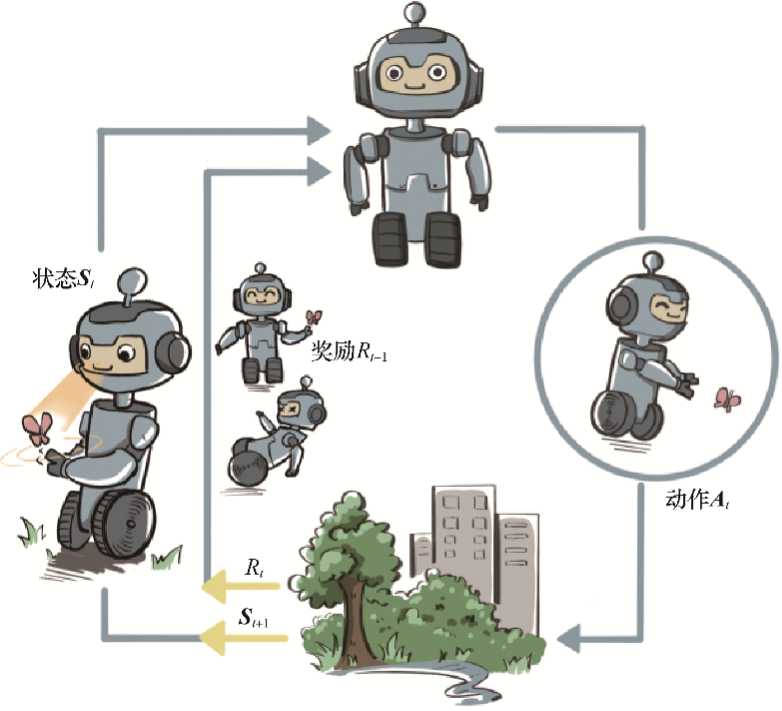
\includegraphics[width=0.8\linewidth]{./assets/11.da5ee18f.png}
% img

图1-1 强化学习中智能体和环境之间的迭代式交互

智能体有 3 种关键要素：\colorbox{mdc2}{感知、决策和奖励}。

\begin{itemize}
  \item 感知。智能体在某种程度上感知环境的状态，从而知道自己所处的现状。例如，下围棋的智能体感知当前的棋盘情况；无人车感知周围道路的车辆、行人和红绿灯等情况；机器狗通过摄像头感知面前的图像，通过脚底的力学传感器来感知地面的摩擦功率和倾斜度等情况。
  \item 智能体根据当前的状态计算出达到目标需要采取的动作的过程叫作决策。例如，针对当前的棋盘决定下一颗落子的位置；针对当前的路况，无人车计算出方向盘的角度和刹车、油门的力度；针对当前收集到的视觉和力觉信号，机器狗给出4条腿的齿轮的角速度。策略是智能体最终体现出的智能形式，是不同智能体之间的核心区别。
  \item 奖励。环境根据状态和智能体采取的动作，产生一个标量信号作为奖励反馈。这个标量信号衡量智能体这一轮动作的好坏。例如，围棋博弈是否胜利；无人车是否安全、平稳且快速地行驶；机器狗是否在前进而没有摔倒。最大化累积奖励期望是智能体提升策略的目标，也是衡量智能体策略好坏的关键指标。
\end{itemize}

强化学习和有监督学习在形式上有不少区别。决策任务往往涉及多轮交互，预测任务总是单轮的独立任务；如果决策也是单轮的，它可以转化为“判别最优动作”的预测任务。决策是多轮的，智能体在每轮做决策时就得考虑未来环境的变化，\colorbox{mdc1}{所以当前轮带来最大奖励反馈的动作，在长期来看并不一定是最优的}。

\subsection{强化学习的环境}

强化学习的智能体是在\colorbox{mdc1}{和一个动态环境的交互}中完成序贯决策的。一个环境是动态的，意思是它会随着某些因素不断演变，这在数学和物理中往往\colorbox{mdc1}{用随机过程来刻画}。生活里几乎所有的系统都在演变：一座城市的交通、一片湖中的生态、一场足球比赛、一个星系。随机过程最关键的要素是状态以及状态转移的条件概率分布。一个微粒在水中的布朗运动，可以由它的起始位置以及下一刻位置相对当前位置的条件概率分布来刻画。

如果在环境这样一个自身演变的随机过程中加入一个外来的干扰因素，即智能体的动作，那么环境的下一刻状态的概率分布将由当前状态和智能体的动作来共同决定，用最简单的数学公式表示则是

\[
下一状态\approx P(\cdot |当前状态,智能体的动作)
\]

动作作用到环境里，环境的状态随之改变，智能体再在新状态下给出下一步决策。

\colorbox{mdc1}{与面向决策任务的智能体进行交互的环境是一个动态的随机过程}，未来状态的分布由当前状态和智能体决策的动作共同决定。每一轮状态转移都伴随两方面的随机性：

\colorbox{mdc1}{一是智能体决策的动作的随机性，二是环境基于当前状态和智能体动作来采样下一刻状态的随机性。}

在动态随机过程里学习和在固定数据分布下学习，是两件很不同的事。

\subsection{强化学习的目标}

在上述动态环境下，智能体和环境每交互一次，环境就产生一个奖励信号，通常由\colorbox{mdc1}{实数标量}表示。奖励信号是当前状态或动作好坏的及时反馈，好比游戏里一次操作拿到的分数。每一轮的奖励可以累加，形成智能体的整体回报（return），好比一盘游戏的最终得分。环境是动态的：即使环境、策略和初始状态都不变，交互结果也很可能不同，回报也会不同。所以强化学习关注回报的期望，并把它定义为价值（value），这就是智能体要优化的目标。

价值的计算有些复杂，因为要对每一轮动作的概率分布和环境状态转移的概率分布做积分。强化学习和有监督学习的目标其实一致：都在某个数据分布下优化一个分数值的期望。但优化途径不同。

\subsection{强化学习中的数据}

从数据层面看，两者的区别更清楚。

有监督学习的任务建立在从\colorbox{mdc1}{给定的数据分布}中采样得到的训练数据集上，通过优化在训练数据集中设定的目标函数（如最小化预测误差）来找到模型的最优参数。这里，\colorbox{mdc1}{训练数据集背后的数据分布是完全不变的}。

在强化学习中，数据是在智能体与环境交互的过程中得到的。如果智能体不采取某个决策动作，那么该动作对应的数据就永远无法被观测到，所以当前智能体的训练数据来自之前智能体的决策结果。因此，\colorbox{mdc1}{智能体的策略不同，与环境交互所产生的数据分布就不同}，如图1-2所示。

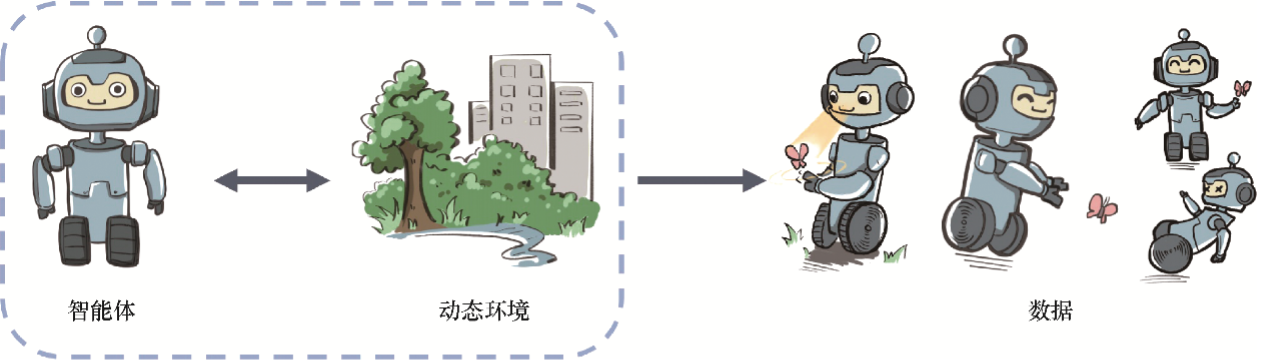
\includegraphics[width=0.8\linewidth]{./assets/12.683654d1.png}
% img

图1-2 强化学习中智能体与环境交互产生相应的数据分布

\colorbox{mdc1}{强化学习中有一个关于数据分布的概念，叫作占用度量（occupancy measure)}。它的数学定义和性质放到第3章，这里只做简要陈述：\colorbox{mdc1}{归一化的占用度量用于衡量在一个智能体决策与一个动态环境的交互过程中，采样到一个具体的状态动作对（state-action pair）的概率分布}。

占用度量有一个很重要的性质：给定两个策略及其与一个动态环境交互得到的两个占用度量，那么当且仅当这两个占用度量相同时，这两个策略相同。也就是说，如果一个智能体的策略有所改变，那么它和环境交互得到的占用度量也会相应改变。

由这个性质可以推出强化学习的两个基本认识。

\begin{itemize}
  \item 强化学习的策略在训练中会不断更新，其对应的数据分布（即占用度量）也会相应地改变。因此，强化学习的一大难点就在于，智能体看到的数据分布是随着智能体的学习而不断发生改变的。
  \item 由于奖励建立在状态动作对之上，\colorbox{mdc1}{一个策略对应的价值其实就是一个占用度量下对应的奖励的期望}，因此寻找最优策略对应着寻找最优占用度量。
\end{itemize}

\subsection{强化学习的独特性}

回过头看有监督学习和强化学习的区别。

对于一般的有监督学习任务，我们的目标是找到一个最优的模型函数，使其在训练数据集上最小化一个给定的损失函数。在训练数据独立同分布的假设下，这个优化目标表示最小化模型在整个数据分布上的泛化误差（generalization error），用简要的公式可以概括为：

最优模型模型特征，标签数据分布损失函数标签，模型特征

相比之下，强化学习任务的最终优化目标是最大化智能体策略在和动态环境交互过程中的价值。根据1.5节的分析，策略的价值可以等价转换成奖励函数在策略的占用度量上的期望，即：

最优策略策略状态，动作策略的占用度量奖励函数状态，动作

两个优化目标相似，都是在优化某个数据分布下的分数值期望。区别在优化途径。有监督学习直接优化模型对数据特征的输出，数据分布不变；强化学习改变策略，由此改变智能体和环境交互产生的数据分布，奖励函数不变。前者是在给定数据分布下找一个损失期望最小的模型，后者是在动态环境里找一个能产生最优数据分布的策略，即最大化该分布下给定奖励函数的期望。

\subsection{小结}

强化学习通常比一般的有监督学习难。策略一变，交互产生的数据分布就跟着变；这种变化高度复杂、不可追踪，往往写不成显式公式。像一个混沌系统：给定初始设置，也拿不到最终状态的分布。有监督学习没有这层麻烦。
